\documentclass[twoside]{book}

% Packages required by doxygen
\usepackage{fixltx2e}
\usepackage{calc}
\usepackage{doxygen}
\usepackage[export]{adjustbox} % also loads graphicx
\usepackage{graphicx}
\usepackage[utf8]{inputenc}
\usepackage{makeidx}
\usepackage{multicol}
\usepackage{multirow}
\PassOptionsToPackage{warn}{textcomp}
\usepackage{textcomp}
\usepackage[nointegrals]{wasysym}
\usepackage[table]{xcolor}

% Font selection
\usepackage[T1]{fontenc}
\usepackage[scaled=.90]{helvet}
\usepackage{courier}
\usepackage{amssymb}
\usepackage{sectsty}
\renewcommand{\familydefault}{\sfdefault}
\allsectionsfont{%
  \fontseries{bc}\selectfont%
  \color{darkgray}%
}
\renewcommand{\DoxyLabelFont}{%
  \fontseries{bc}\selectfont%
  \color{darkgray}%
}
\newcommand{\+}{\discretionary{\mbox{\scriptsize$\hookleftarrow$}}{}{}}

% Page & text layout
\usepackage{geometry}
\geometry{%
  a4paper,%
  top=2.5cm,%
  bottom=2.5cm,%
  left=2.5cm,%
  right=2.5cm%
}
\tolerance=750
\hfuzz=15pt
\hbadness=750
\setlength{\emergencystretch}{15pt}
\setlength{\parindent}{0cm}
\setlength{\parskip}{3ex plus 2ex minus 2ex}
\makeatletter
\renewcommand{\paragraph}{%
  \@startsection{paragraph}{4}{0ex}{-1.0ex}{1.0ex}{%
    \normalfont\normalsize\bfseries\SS@parafont%
  }%
}
\renewcommand{\subparagraph}{%
  \@startsection{subparagraph}{5}{0ex}{-1.0ex}{1.0ex}{%
    \normalfont\normalsize\bfseries\SS@subparafont%
  }%
}
\makeatother

% Headers & footers
\usepackage{fancyhdr}
\pagestyle{fancyplain}
\fancyhead[LE]{\fancyplain{}{\bfseries\thepage}}
\fancyhead[CE]{\fancyplain{}{}}
\fancyhead[RE]{\fancyplain{}{\bfseries\leftmark}}
\fancyhead[LO]{\fancyplain{}{\bfseries\rightmark}}
\fancyhead[CO]{\fancyplain{}{}}
\fancyhead[RO]{\fancyplain{}{\bfseries\thepage}}
\fancyfoot[LE]{\fancyplain{}{}}
\fancyfoot[CE]{\fancyplain{}{}}
\fancyfoot[RE]{\fancyplain{}{\bfseries\scriptsize Generated by Doxygen }}
\fancyfoot[LO]{\fancyplain{}{\bfseries\scriptsize Generated by Doxygen }}
\fancyfoot[CO]{\fancyplain{}{}}
\fancyfoot[RO]{\fancyplain{}{}}
\renewcommand{\footrulewidth}{0.4pt}
\renewcommand{\chaptermark}[1]{%
  \markboth{#1}{}%
}
\renewcommand{\sectionmark}[1]{%
  \markright{\thesection\ #1}%
}

% Indices & bibliography
\usepackage{natbib}
\usepackage[titles]{tocloft}
\setcounter{tocdepth}{3}
\setcounter{secnumdepth}{5}
\makeindex

% Hyperlinks (required, but should be loaded last)
\usepackage{ifpdf}
\ifpdf
  \usepackage[pdftex,pagebackref=true]{hyperref}
\else
  \usepackage[ps2pdf,pagebackref=true]{hyperref}
\fi
\hypersetup{%
  colorlinks=true,%
  linkcolor=blue,%
  citecolor=blue,%
  unicode%
}

% Custom commands
\newcommand{\clearemptydoublepage}{%
  \newpage{\pagestyle{empty}\cleardoublepage}%
}

\usepackage{caption}
\captionsetup{labelsep=space,justification=centering,font={bf},singlelinecheck=off,skip=4pt,position=top}

%===== C O N T E N T S =====

\begin{document}

% Titlepage & ToC
\hypersetup{pageanchor=false,
             bookmarksnumbered=true,
             pdfencoding=unicode
            }
\pagenumbering{alph}
\begin{titlepage}
\vspace*{7cm}
\begin{center}%
{\Large Example Python Doxygen }\\
\vspace*{1cm}
{\large Generated by Doxygen 1.8.13}\\
\end{center}
\end{titlepage}
\clearemptydoublepage
\pagenumbering{roman}
\tableofcontents
\clearemptydoublepage
\pagenumbering{arabic}
\hypersetup{pageanchor=true}

%--- Begin generated contents ---
\chapter{Namespace Index}
\section{Packages}
Here are the packages with brief descriptions (if available)\+:\begin{DoxyCompactList}
\item\contentsline{section}{\hyperlink{namespacesrc}{src} }{\pageref{namespacesrc}}{}
\item\contentsline{section}{\hyperlink{namespacesrc_1_1a}{src.\+a} }{\pageref{namespacesrc_1_1a}}{}
\item\contentsline{section}{\hyperlink{namespacesrc_1_1b}{src.\+b} }{\pageref{namespacesrc_1_1b}}{}
\item\contentsline{section}{\hyperlink{namespacesrc_1_1my__class}{src.\+my\+\_\+class} }{\pageref{namespacesrc_1_1my__class}}{}
\item\contentsline{section}{\hyperlink{namespacesrc_1_1my__other__class}{src.\+my\+\_\+other\+\_\+class} }{\pageref{namespacesrc_1_1my__other__class}}{}
\end{DoxyCompactList}

\chapter{Hierarchical Index}
\section{Class Hierarchy}
This inheritance list is sorted roughly, but not completely, alphabetically\+:\begin{DoxyCompactList}
\item object\begin{DoxyCompactList}
\item \contentsline{section}{My\+Other\+Class}{\pageref{classsrc_1_1my__other__class_1_1MyOtherClass}}{}
\begin{DoxyCompactList}
\item \contentsline{section}{My\+Class}{\pageref{classsrc_1_1my__class_1_1MyClass}}{}
\end{DoxyCompactList}
\end{DoxyCompactList}
\end{DoxyCompactList}

\chapter{Class Index}
\section{Class List}
Here are the classes, structs, unions and interfaces with brief descriptions\+:\begin{DoxyCompactList}
\item\contentsline{section}{\hyperlink{classsrc_1_1my__class_1_1MyClass}{My\+Class} }{\pageref{classsrc_1_1my__class_1_1MyClass}}{}
\item\contentsline{section}{\hyperlink{classsrc_1_1my__other__class_1_1MyOtherClass}{My\+Other\+Class} }{\pageref{classsrc_1_1my__other__class_1_1MyOtherClass}}{}
\end{DoxyCompactList}

\chapter{File Index}
\section{File List}
Here is a list of all files with brief descriptions\+:\begin{DoxyCompactList}
\item\contentsline{section}{/home/wmboler/\+Tutorials/\+Python\+Doxygen/src/\hyperlink{____init_____8py}{\+\_\+\+\_\+init\+\_\+\+\_\+.\+py} }{\pageref{____init_____8py}}{}
\item\contentsline{section}{/home/wmboler/\+Tutorials/\+Python\+Doxygen/src/\hyperlink{a_8py}{a.\+py} }{\pageref{a_8py}}{}
\item\contentsline{section}{/home/wmboler/\+Tutorials/\+Python\+Doxygen/src/\hyperlink{b_8py}{b.\+py} }{\pageref{b_8py}}{}
\item\contentsline{section}{/home/wmboler/\+Tutorials/\+Python\+Doxygen/src/\hyperlink{my__class_8py}{my\+\_\+class.\+py} }{\pageref{my__class_8py}}{}
\item\contentsline{section}{/home/wmboler/\+Tutorials/\+Python\+Doxygen/src/\hyperlink{my__other__class_8py}{my\+\_\+other\+\_\+class.\+py} }{\pageref{my__other__class_8py}}{}
\end{DoxyCompactList}

\chapter{Namespace Documentation}
\hypertarget{namespacesrc}{}\section{src Namespace Reference}
\label{namespacesrc}\index{src@{src}}
\subsection*{Namespaces}
\begin{DoxyCompactItemize}
\item 
 \hyperlink{namespacesrc_1_1a}{a}
\item 
 \hyperlink{namespacesrc_1_1b}{b}
\item 
 \hyperlink{namespacesrc_1_1my__class}{my\+\_\+class}
\item 
 \hyperlink{namespacesrc_1_1my__other__class}{my\+\_\+other\+\_\+class}
\end{DoxyCompactItemize}

\hypertarget{namespacesrc_1_1a}{}\section{src.\+a Namespace Reference}
\label{namespacesrc_1_1a}\index{src.\+a@{src.\+a}}
\subsection*{Functions}
\begin{DoxyCompactItemize}
\item 
def \hyperlink{namespacesrc_1_1a_ab6ca8696e646cc990881db753c957101}{a} ()
\end{DoxyCompactItemize}


\subsection{Detailed Description}
\begin{DoxyVerb}Prints MyClass with n=5
\end{DoxyVerb}
 

\subsection{Function Documentation}
\mbox{\Hypertarget{namespacesrc_1_1a_ab6ca8696e646cc990881db753c957101}\label{namespacesrc_1_1a_ab6ca8696e646cc990881db753c957101}} 
\index{src\+::a@{src\+::a}!a@{a}}
\index{a@{a}!src\+::a@{src\+::a}}
\subsubsection{\texorpdfstring{a()}{a()}}
{\footnotesize\ttfamily def src.\+a.\+a (\begin{DoxyParamCaption}{ }\end{DoxyParamCaption})}

\begin{DoxyVerb}Prints sum of two arrays with n=5
\end{DoxyVerb}
 
\hypertarget{namespacesrc_1_1b}{}\section{src.\+b Namespace Reference}
\label{namespacesrc_1_1b}\index{src.\+b@{src.\+b}}
\subsection*{Functions}
\begin{DoxyCompactItemize}
\item 
def \hyperlink{namespacesrc_1_1b_afee0552d4bea354c388fd3bfacc91440}{b} ()
\end{DoxyCompactItemize}


\subsection{Detailed Description}
\begin{DoxyVerb}Prints MyClass with n=10
\end{DoxyVerb}
 

\subsection{Function Documentation}
\mbox{\Hypertarget{namespacesrc_1_1b_afee0552d4bea354c388fd3bfacc91440}\label{namespacesrc_1_1b_afee0552d4bea354c388fd3bfacc91440}} 
\index{src\+::b@{src\+::b}!b@{b}}
\index{b@{b}!src\+::b@{src\+::b}}
\subsubsection{\texorpdfstring{b()}{b()}}
{\footnotesize\ttfamily def src.\+b.\+b (\begin{DoxyParamCaption}{ }\end{DoxyParamCaption})}

\begin{DoxyVerb}Prints sum of two arrays with n=10
\end{DoxyVerb}
 
\hypertarget{namespacesrc_1_1my__class}{}\section{src.\+my\+\_\+class Namespace Reference}
\label{namespacesrc_1_1my__class}\index{src.\+my\+\_\+class@{src.\+my\+\_\+class}}
\subsection*{Classes}
\begin{DoxyCompactItemize}
\item 
class \hyperlink{classsrc_1_1my__class_1_1MyClass}{My\+Class}
\end{DoxyCompactItemize}


\subsection{Detailed Description}
\begin{DoxyVerb}An example class that randomly generates two arrays
and adds them together.  It provides an example to show
with Doxygen and Sphinx, and does nothing special.
\end{DoxyVerb}
 
\hypertarget{namespacesrc_1_1my__other__class}{}\section{src.\+my\+\_\+other\+\_\+class Namespace Reference}
\label{namespacesrc_1_1my__other__class}\index{src.\+my\+\_\+other\+\_\+class@{src.\+my\+\_\+other\+\_\+class}}
\subsection*{Classes}
\begin{DoxyCompactItemize}
\item 
class \hyperlink{classsrc_1_1my__other__class_1_1MyOtherClass}{My\+Other\+Class}
\end{DoxyCompactItemize}


\subsection{Detailed Description}
\begin{DoxyVerb}I want to add some complexity to our MyClass
\end{DoxyVerb}
 
\chapter{Class Documentation}
\hypertarget{classsrc_1_1my__class_1_1MyClass}{}\section{My\+Class Class Reference}
\label{classsrc_1_1my__class_1_1MyClass}\index{My\+Class@{My\+Class}}


Inheritance diagram for My\+Class\+:\nopagebreak
\begin{figure}[H]
\begin{center}
\leavevmode
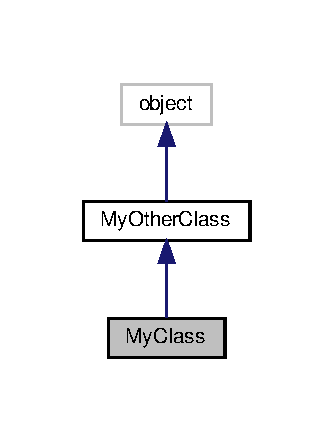
\includegraphics[width=160pt]{classsrc_1_1my__class_1_1MyClass__inherit__graph}
\end{center}
\end{figure}


Collaboration diagram for My\+Class\+:\nopagebreak
\begin{figure}[H]
\begin{center}
\leavevmode
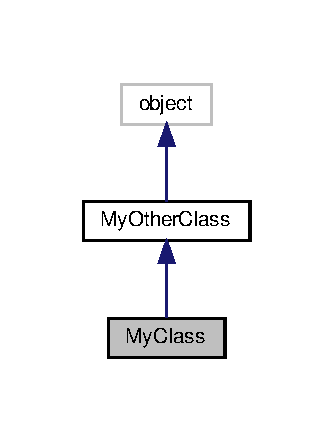
\includegraphics[width=160pt]{classsrc_1_1my__class_1_1MyClass__coll__graph}
\end{center}
\end{figure}
\subsection*{Public Member Functions}
\begin{DoxyCompactItemize}
\item 
def \hyperlink{classsrc_1_1my__class_1_1MyClass_a01f7e43ceaf00de636b0e2fa32459c80}{\+\_\+\+\_\+init\+\_\+\+\_\+} (self, n=5)
\item 
def \hyperlink{classsrc_1_1my__class_1_1MyClass_af06166582a4454b37fc37239d03ec7da}{calc} (self)
\end{DoxyCompactItemize}
\subsection*{Public Attributes}
\begin{DoxyCompactItemize}
\item 
\hyperlink{classsrc_1_1my__class_1_1MyClass_a4124bc0a9335c27f086f24ba207a4912}{a}
\item 
\hyperlink{classsrc_1_1my__class_1_1MyClass_a21ad0bd836b90d08f4cf640b4c298e7c}{b}
\item 
\hyperlink{classsrc_1_1my__class_1_1MyClass_ae0323a9039add2978bf5b49550572c7c}{c}
\end{DoxyCompactItemize}


\subsection{Detailed Description}
\begin{DoxyVerb}A class that randomly generates 2 arrays and adds them together.
\end{DoxyVerb}
 

\subsection{Constructor \& Destructor Documentation}
\mbox{\Hypertarget{classsrc_1_1my__class_1_1MyClass_a01f7e43ceaf00de636b0e2fa32459c80}\label{classsrc_1_1my__class_1_1MyClass_a01f7e43ceaf00de636b0e2fa32459c80}} 
\index{src\+::my\+\_\+class\+::\+My\+Class@{src\+::my\+\_\+class\+::\+My\+Class}!\+\_\+\+\_\+init\+\_\+\+\_\+@{\+\_\+\+\_\+init\+\_\+\+\_\+}}
\index{\+\_\+\+\_\+init\+\_\+\+\_\+@{\+\_\+\+\_\+init\+\_\+\+\_\+}!src\+::my\+\_\+class\+::\+My\+Class@{src\+::my\+\_\+class\+::\+My\+Class}}
\subsubsection{\texorpdfstring{\+\_\+\+\_\+init\+\_\+\+\_\+()}{\_\_init\_\_()}}
{\footnotesize\ttfamily def \+\_\+\+\_\+init\+\_\+\+\_\+ (\begin{DoxyParamCaption}\item[{}]{self,  }\item[{}]{n = {\ttfamily 5} }\end{DoxyParamCaption})}

\begin{DoxyVerb}Instantiates two arrays

@param n size of arrays
\end{DoxyVerb}
 

\subsection{Member Function Documentation}
\mbox{\Hypertarget{classsrc_1_1my__class_1_1MyClass_af06166582a4454b37fc37239d03ec7da}\label{classsrc_1_1my__class_1_1MyClass_af06166582a4454b37fc37239d03ec7da}} 
\index{src\+::my\+\_\+class\+::\+My\+Class@{src\+::my\+\_\+class\+::\+My\+Class}!calc@{calc}}
\index{calc@{calc}!src\+::my\+\_\+class\+::\+My\+Class@{src\+::my\+\_\+class\+::\+My\+Class}}
\subsubsection{\texorpdfstring{calc()}{calc()}}
{\footnotesize\ttfamily def calc (\begin{DoxyParamCaption}\item[{}]{self }\end{DoxyParamCaption})}

\begin{DoxyVerb}Adds two arrays a and b and returns sum

@return np.array Sum of 'a' + 'b'
\end{DoxyVerb}
 

\subsection{Member Data Documentation}
\mbox{\Hypertarget{classsrc_1_1my__class_1_1MyClass_a4124bc0a9335c27f086f24ba207a4912}\label{classsrc_1_1my__class_1_1MyClass_a4124bc0a9335c27f086f24ba207a4912}} 
\index{src\+::my\+\_\+class\+::\+My\+Class@{src\+::my\+\_\+class\+::\+My\+Class}!a@{a}}
\index{a@{a}!src\+::my\+\_\+class\+::\+My\+Class@{src\+::my\+\_\+class\+::\+My\+Class}}
\subsubsection{\texorpdfstring{a}{a}}
{\footnotesize\ttfamily a}

\mbox{\Hypertarget{classsrc_1_1my__class_1_1MyClass_a21ad0bd836b90d08f4cf640b4c298e7c}\label{classsrc_1_1my__class_1_1MyClass_a21ad0bd836b90d08f4cf640b4c298e7c}} 
\index{src\+::my\+\_\+class\+::\+My\+Class@{src\+::my\+\_\+class\+::\+My\+Class}!b@{b}}
\index{b@{b}!src\+::my\+\_\+class\+::\+My\+Class@{src\+::my\+\_\+class\+::\+My\+Class}}
\subsubsection{\texorpdfstring{b}{b}}
{\footnotesize\ttfamily b}

\mbox{\Hypertarget{classsrc_1_1my__class_1_1MyClass_ae0323a9039add2978bf5b49550572c7c}\label{classsrc_1_1my__class_1_1MyClass_ae0323a9039add2978bf5b49550572c7c}} 
\index{src\+::my\+\_\+class\+::\+My\+Class@{src\+::my\+\_\+class\+::\+My\+Class}!c@{c}}
\index{c@{c}!src\+::my\+\_\+class\+::\+My\+Class@{src\+::my\+\_\+class\+::\+My\+Class}}
\subsubsection{\texorpdfstring{c}{c}}
{\footnotesize\ttfamily c}



The documentation for this class was generated from the following file\+:\begin{DoxyCompactItemize}
\item 
/home/wmboler/\+Tutorials/\+Python\+Doxygen/example\+\_\+package/src/\hyperlink{my__class_8py}{my\+\_\+class.\+py}\end{DoxyCompactItemize}

\hypertarget{classsrc_1_1my__other__class_1_1MyOtherClass}{}\section{My\+Other\+Class Class Reference}
\label{classsrc_1_1my__other__class_1_1MyOtherClass}\index{My\+Other\+Class@{My\+Other\+Class}}


Inheritance diagram for My\+Other\+Class\+:\nopagebreak
\begin{figure}[H]
\begin{center}
\leavevmode
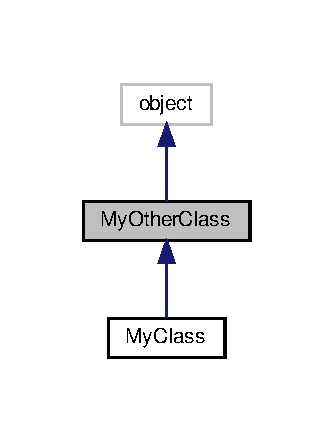
\includegraphics[width=160pt]{classsrc_1_1my__other__class_1_1MyOtherClass__inherit__graph}
\end{center}
\end{figure}


Collaboration diagram for My\+Other\+Class\+:\nopagebreak
\begin{figure}[H]
\begin{center}
\leavevmode
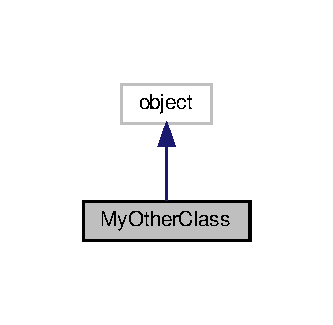
\includegraphics[width=160pt]{classsrc_1_1my__other__class_1_1MyOtherClass__coll__graph}
\end{center}
\end{figure}
\subsection*{Public Member Functions}
\begin{DoxyCompactItemize}
\item 
def \hyperlink{classsrc_1_1my__other__class_1_1MyOtherClass_ae64f0875afe3067b97ba370b354b9213}{\+\_\+\+\_\+init\+\_\+\+\_\+} (self)
\item 
def \hyperlink{classsrc_1_1my__other__class_1_1MyOtherClass_a711fec1561ace90a200ff0eaafeaee49}{print} (self)
\end{DoxyCompactItemize}
\subsection*{Public Attributes}
\begin{DoxyCompactItemize}
\item 
\hyperlink{classsrc_1_1my__other__class_1_1MyOtherClass_ae0323a9039add2978bf5b49550572c7c}{c}
\end{DoxyCompactItemize}


\subsection{Detailed Description}
\begin{DoxyVerb}This is just another class that adds complexity to MyClass
\end{DoxyVerb}
 

\subsection{Constructor \& Destructor Documentation}
\mbox{\Hypertarget{classsrc_1_1my__other__class_1_1MyOtherClass_ae64f0875afe3067b97ba370b354b9213}\label{classsrc_1_1my__other__class_1_1MyOtherClass_ae64f0875afe3067b97ba370b354b9213}} 
\index{src\+::my\+\_\+other\+\_\+class\+::\+My\+Other\+Class@{src\+::my\+\_\+other\+\_\+class\+::\+My\+Other\+Class}!\+\_\+\+\_\+init\+\_\+\+\_\+@{\+\_\+\+\_\+init\+\_\+\+\_\+}}
\index{\+\_\+\+\_\+init\+\_\+\+\_\+@{\+\_\+\+\_\+init\+\_\+\+\_\+}!src\+::my\+\_\+other\+\_\+class\+::\+My\+Other\+Class@{src\+::my\+\_\+other\+\_\+class\+::\+My\+Other\+Class}}
\subsubsection{\texorpdfstring{\+\_\+\+\_\+init\+\_\+\+\_\+()}{\_\_init\_\_()}}
{\footnotesize\ttfamily def \+\_\+\+\_\+init\+\_\+\+\_\+ (\begin{DoxyParamCaption}\item[{}]{self }\end{DoxyParamCaption})}



\subsection{Member Function Documentation}
\mbox{\Hypertarget{classsrc_1_1my__other__class_1_1MyOtherClass_a711fec1561ace90a200ff0eaafeaee49}\label{classsrc_1_1my__other__class_1_1MyOtherClass_a711fec1561ace90a200ff0eaafeaee49}} 
\index{src\+::my\+\_\+other\+\_\+class\+::\+My\+Other\+Class@{src\+::my\+\_\+other\+\_\+class\+::\+My\+Other\+Class}!print@{print}}
\index{print@{print}!src\+::my\+\_\+other\+\_\+class\+::\+My\+Other\+Class@{src\+::my\+\_\+other\+\_\+class\+::\+My\+Other\+Class}}
\subsubsection{\texorpdfstring{print()}{print()}}
{\footnotesize\ttfamily def print (\begin{DoxyParamCaption}\item[{}]{self }\end{DoxyParamCaption})}

\begin{DoxyVerb}Prints the internal self.c
\end{DoxyVerb}
 

\subsection{Member Data Documentation}
\mbox{\Hypertarget{classsrc_1_1my__other__class_1_1MyOtherClass_ae0323a9039add2978bf5b49550572c7c}\label{classsrc_1_1my__other__class_1_1MyOtherClass_ae0323a9039add2978bf5b49550572c7c}} 
\index{src\+::my\+\_\+other\+\_\+class\+::\+My\+Other\+Class@{src\+::my\+\_\+other\+\_\+class\+::\+My\+Other\+Class}!c@{c}}
\index{c@{c}!src\+::my\+\_\+other\+\_\+class\+::\+My\+Other\+Class@{src\+::my\+\_\+other\+\_\+class\+::\+My\+Other\+Class}}
\subsubsection{\texorpdfstring{c}{c}}
{\footnotesize\ttfamily c}



The documentation for this class was generated from the following file\+:\begin{DoxyCompactItemize}
\item 
/home/wmboler/\+Tutorials/\+Python\+Doxygen/example\+\_\+package/src/\hyperlink{my__other__class_8py}{my\+\_\+other\+\_\+class.\+py}\end{DoxyCompactItemize}

\chapter{File Documentation}
\hypertarget{____init_____8py}{}\section{/home/wmboler/\+Tutorials/\+Python\+Doxygen/src/\+\_\+\+\_\+init\+\_\+\+\_\+.py File Reference}
\label{____init_____8py}\index{/home/wmboler/\+Tutorials/\+Python\+Doxygen/src/\+\_\+\+\_\+init\+\_\+\+\_\+.\+py@{/home/wmboler/\+Tutorials/\+Python\+Doxygen/src/\+\_\+\+\_\+init\+\_\+\+\_\+.\+py}}
\subsection*{Namespaces}
\begin{DoxyCompactItemize}
\item 
 \hyperlink{namespacesrc}{src}
\end{DoxyCompactItemize}

\hypertarget{a_8py}{}\section{/home/wmboler/\+Tutorials/\+Python\+Doxygen/src/a.py File Reference}
\label{a_8py}\index{/home/wmboler/\+Tutorials/\+Python\+Doxygen/src/a.\+py@{/home/wmboler/\+Tutorials/\+Python\+Doxygen/src/a.\+py}}
\subsection*{Namespaces}
\begin{DoxyCompactItemize}
\item 
 \hyperlink{namespacesrc_1_1a}{src.\+a}
\end{DoxyCompactItemize}
\subsection*{Functions}
\begin{DoxyCompactItemize}
\item 
def \hyperlink{namespacesrc_1_1a_ab6ca8696e646cc990881db753c957101}{a} ()
\end{DoxyCompactItemize}

\hypertarget{b_8py}{}\section{/home/wmboler/\+Tutorials/\+Python\+Doxygen/src/b.py File Reference}
\label{b_8py}\index{/home/wmboler/\+Tutorials/\+Python\+Doxygen/src/b.\+py@{/home/wmboler/\+Tutorials/\+Python\+Doxygen/src/b.\+py}}
\subsection*{Namespaces}
\begin{DoxyCompactItemize}
\item 
 \hyperlink{namespacesrc_1_1b}{src.\+b}
\end{DoxyCompactItemize}
\subsection*{Functions}
\begin{DoxyCompactItemize}
\item 
def \hyperlink{namespacesrc_1_1b_afee0552d4bea354c388fd3bfacc91440}{b} ()
\end{DoxyCompactItemize}

\hypertarget{my__class_8py}{}\section{/home/wmboler/\+Tutorials/\+Python\+Doxygen/example\+\_\+package/src/my\+\_\+class.py File Reference}
\label{my__class_8py}\index{/home/wmboler/\+Tutorials/\+Python\+Doxygen/example\+\_\+package/src/my\+\_\+class.\+py@{/home/wmboler/\+Tutorials/\+Python\+Doxygen/example\+\_\+package/src/my\+\_\+class.\+py}}
\subsection*{Classes}
\begin{DoxyCompactItemize}
\item 
class \hyperlink{classsrc_1_1my__class_1_1MyClass}{My\+Class}
\end{DoxyCompactItemize}
\subsection*{Namespaces}
\begin{DoxyCompactItemize}
\item 
 \hyperlink{namespacesrc_1_1my__class}{src.\+my\+\_\+class}
\end{DoxyCompactItemize}

\hypertarget{my__other__class_8py}{}\section{/home/wmboler/\+Tutorials/\+Python\+Doxygen/src/my\+\_\+other\+\_\+class.py File Reference}
\label{my__other__class_8py}\index{/home/wmboler/\+Tutorials/\+Python\+Doxygen/src/my\+\_\+other\+\_\+class.\+py@{/home/wmboler/\+Tutorials/\+Python\+Doxygen/src/my\+\_\+other\+\_\+class.\+py}}
\subsection*{Classes}
\begin{DoxyCompactItemize}
\item 
class \hyperlink{classsrc_1_1my__other__class_1_1MyOtherClass}{My\+Other\+Class}
\end{DoxyCompactItemize}
\subsection*{Namespaces}
\begin{DoxyCompactItemize}
\item 
 \hyperlink{namespacesrc_1_1my__other__class}{src.\+my\+\_\+other\+\_\+class}
\end{DoxyCompactItemize}

%--- End generated contents ---

% Index
\backmatter
\newpage
\phantomsection
\clearemptydoublepage
\addcontentsline{toc}{chapter}{Index}
\printindex

\end{document}
